\chapter{Fixed-Encoding Networks}
\chplabel{nef}

\newcommand{\Dec}{\Omega}
\newcommand{\dec}{\vect \omega}

%% The first type of deep network we will examine in this thesis
%% are what I call \emph{fixed-encoding networks}.
%% These networks are so-named because all weights going into hidden units---%
%% that is, all the weights that define the network's encoding of the input---%
%% are fixed.
%% The only weights that are learned are the \emph{decoding} weights,
%% that is the weights that map from the final layer to the output units.
%% Furthermore, using a squared error metric results in a linear system
%% with a closed-form linear solution,
%% which can be solved much more efficiently than nonlinear problems.
%% Essentially, it amounts to linear regression
%% over a fixed set of basis vectors.

The first type of deep network I examine in this thesis
is what I call \emph{fixed-encoding networks}.
These networks are so-named because all weights going into hidden units---%
that is, all the weights that define the network's encoding of the input---%
are fixed.
The only weights that are learned are the \emph{decoding} weights,
that is the weights that map from the final layer to the output units.

Specifically, I focus on single-layer feedforward networks (SLFNs)
with a linear $\to$ nonlinear $\to$ linear structure.
That is, these networks have a multilayer perceptron (MLP) structure,
with a linear input layer, a single nonlinear hidden layer,
and a linear output layer.
Unlike most ANNs, however, they have the additional qualification
that the weights from the input layer to the hidden layer---%
which I call the \emph{encoders}---are fixed.
Only the weights from the hidden layer to the output---%
the \emph{decoders}---are learned.
This specific type of network has often gone by the name
``flat network'' \parencite{Pao1992,Chen1999}.

This specific type of network is of interest to me
because it is at the core of the Neural Engineering Framework (NEF) \parencite{Eliasmith2003}.
The NEF describes how such single-layer networks
can be combined to create very large multilayer networks of spiking neurons.
This chapter expands on two aspects of these networks
that have not been well covered by \textcite{Eliasmith2003}
or subsequent works with the NEF:
how the choice of encoders and the methods used to find decoders
affect the performance of the network,
as applied to object classification.

%% The structure typically used by fixed-encoding networks is a
%% fixed nonlinear encoding, and an optimized linear decoding.
%% The encoding often consists of only a single hidden layer of neurons:
%% the input is multiplied by a fixed set of linear encoding weights,
%% then passed through a neural nonlinearity.
%% Multi-hidden-layer fixed-encoding networks also exist;
%% these will not be the focus of this chapter,
%% but I will review some of the existing methods.
%% Finally, other encoding methods than linear-nonlinear are possible,
%% such as radial basis functions (RBF);
%% again, these will not be examined in detail.


\section{Background}

According to \textcite{Wang2008},
the idea of a fixed (nonlinear) encoding began with \textcite{Broomhead1988}.
They used a radial basis function network with fixed centres
to provide novel methods for solving the XOR problem.
They found that when the encoding is fixed,
there is a \emph{linear} solution for the decoders.
This is a linear least-squares regression
over a fixed set of basis vectors.
The existence of such a linear solution when using a squared error metric
makes the problem easier to solve than those that require nonlinear methods,
since fast linear-algebra methods apply.
The simplicity of the solution is one of the main features
that has continued to attract researchers to fixed-encoding networks.

\textcite{Pao1989} proposed a multilayer perceptron (MLP) network
with fixed encoding weights,
which is the first network to fit the description of
fixed-encoding SLFN (as described above).
(See \textcite{Wang2008} for a summary of the many follow-up works.)
\textcite{Pao1992} present an iterative solution for the least-squares problem,
likely since this was more efficient on computers of that era.
\textcite{Schmidt1992} proposed the type of random network around the same time,
but showing the direct solution method.
%% Today, direct methods that rely on linear algebra

%% \textcite{Salinas1994}

More recently, fixed-encoding networks have again become popular.
The Neural Engineering Framework (NEF) \parencite{Eliasmith1999,Eliasmith2003}
approaches the problem from a computational-neuroscience perspective,
and uses layers of fixed-encoding networks
to construct biologically-plausible brain models with spiking neurons.
The Extreme Learning Machine (ELM) \parencite{Huang2006} community,
on the other hand, takes a machine learning approach.
Both methods use the same fundamental network structure
and mathematics to solve the problem.
The applications tend to be quite different,
with the NEF targeting dynamic systems performing behavioural tasks
\parencite[\eg/][]{Eliasmith2012},
while the ELM community has focused more on machine learning datasets,
namely MNIST \parencite[\eg/][]{McDonnell2015}.


\subsection{The Neural Engineering Framework}

%% Many of the ideas around fixed-encoding networks
%% were developed and refined as the foundation of the
%% Neural Engineering Framework (NEF) \parencite{Eliasmith2003}.

The Neural Engineering Framework (NEF) \parencite{Eliasmith1999,Eliasmith2003}
has used fixed-encoding networks as a basis
for constructing large biologically-plausible spiking brain models
\parencite[\eg/][]{Eliasmith2012}.
(See \scn{nef} for a more detailed description.)
The key idea behind the NEF is that the combination of
a fixed nonlinear encoding and linear decoding
can be used to represent states,
compute functions (transformations) on these states,
and implement dynamical systems.

One of the strengths of the NEF is that it describes in detail
how a neural system could implement such networks.
First of all, fixed-encoding SLFNs are often chained together,
to create networks with multiple hidden layers.
Since the input and output ``neurons'' of SLFNs are linear,
when chaining them, the decoding weights from the presynaptic layer
and encoding weights from the postsynaptic layer can be combined,
to define direct connection weights between the two layers.
Specifically, the connection weight $W_{ij}$
from presynaptic neuron $i$ (in the first hidden layer)
to postsynaptic neuron $j$ (in the second hidden layer)
is given by
\begin{align}
  W_{ij} = \sum_k^d \Dec_{ik} E_{kj}
\end{align}
where $\Dec$ is the matrix of decoding weights for the first layer,
$\mat E$ is the matrix of encoding weights for the second layer,
and $d$ is the ``dimensionality'' of the connection.
This allows deep networks to be built from many shallow networks,
with each subsequent layer building on the computation done by the previous layers.
A layer can even be recurrently connected to itself in this manner.

Another strength of the NEF is that it typically uses
more biologically plausible neuron models
than machine learning applications,
the most common being the spiking LIF model.
It demonstrates how networks can be trained with rate neurons,
but run in spiking neurons,
and also describes how regularization can improve spiking network performance.

One limitation of the current literature surrounding the NEF
is that classification tasks have not been well examined.
Some NEF models \parencite[\eg/][]{Eliasmith2012}
have used classification components as part of the system,
but these have been trained separately using deep learning methods \parencite{Tang2010a}.
One goal of this chapter is to allow classification functions
to be computed in a similar manner to regression functions in the NEF.


\subsection{Extreme Learning Machines}

Extreme Learning Machines (ELMs) \parencite{Huang2006}
are another framework that use fixed-encoding with SLFNs.
The methods and ideas they use are not novel,
having been previously developed by
\textcite{Broomhead1988}, \textcite{Pao1992}, and \textcite{Eliasmith1999}.
This habit of presenting old wine in new wineskins, so to speak,
has made the ELM authors increasingly controversial,
as more recent publications of theirs still fail to acknowledge
the many papers that come before \parencite[\eg/][]{Huang2012}.
Nevertheless, they have brought about an increased awareness
of some of the capabilities of fixed-encoding networks,
unfortunately under a new name without citing the original sources,
leading to considerable consternation and confusion among other researchers \parencite{Wang2008}.
Here, I focus on the unique contributions from this body of work.

One interesting direction taken by some of the ELM-related literature
is basing the fixed encoding weights on the data,
rather than simply choosing them randomly.\footnote{
  While data-driven encoding weights are new to the ELM community,
  it is common practice with other types of fixed-encoding networks,
  for example the radial basis function (RBF) network.}
\textcite{Tapson2015} pioneered a method called \emph{computed input weights}.
In this method, each hidden neuron targets a particular class:
Given all data points from that class,
the encoding weights for the hidden neuron are given by
those data points times a random sign vector where each element equals $+1$ or $-1$.
This makes each hidden unit excited by some subset of examples from the target class,
and inhibited by other examples from that class.
By having hidden units targeting each of the different classes in the dataset,
the representation of the dataset by the hidden units is
ideally more easily separable by class.

\textcite{Zhu2015} proposed an alternative method for generating
encoding weights based on the dataset.
Their method takes pairs of examples from the dataset,
where the examples in the pair come from different classes.
By making the input weights for each hidden neuron
equal to the difference of one of these pairs,
each hidden neuron (ideally) becomes excited by one class
(or a subset of examples in that class)
and inhibited by another class.
The idea is that this will push the population of hidden neurons
to distinguishing between all pairs of classes.
They call this method the Constrained Difference (CD) method.

\textcite{McDonnell2015} surveys the CIW and CD techniques for encoder generation,
as well as a few others,
and evaluates them on the MNIST dataset,
setting records on this dataset for SLFNs with fixed encoders.

The ELM literature has focused much less on how to choose the decoding weights,
that is, the output weights that map from the hidden neurons to the output categories.
One notable exception is \textcite{Toh2008},
who proposes a weighted least-squares method.
Despite clear advantages of this method,
it has not yet been adopted by most researchers in the ELM field,
who continue to use the traditional least-squares ELM approach.

% Using convolutional filters and linear decoder
More recently, there has been interest in using fixed-encoding methods
to create deeper networks with multiple hidden layers.
\textcite{McDonnell2015a} passed images through a set of convolutional filters,
pooled the output, and then ran the result through a SLFN with random encoders.
The convolutional filters were chosen either as corner and edge filters,
as features from the initial layer of a deep network trained on ImageNet,
or as patches from the centres of the training images.
Using this method, they are able to achieve very strong results
on the MNIST dataset (0.37\% error),
and reasonable results on SVHN (3.96\% error) and CIFAR-10 (24.14\% error),
all without data augmentation.


\section{Encoding methods}
\scnlabel{nef-encoding}

%% One of the key questions with fixed-encoding methods
%% is how to perform the encoding.

The choice of encoding method has a large influence
on the accuracy of fixed-encoding methods.
The optimal encoding method will map the input images
to a space where they are easily linearly separable.

While there are a wide variety of encoding methods available,
here I focus on methods that pass a linear transform of inputs
through an elementwise nonlinearity.
This is the type of architecture most frequently encountered
for a single layer in an ANN:
each hidden unit takes a weighted sum of the inputs,
then passes this through a static nonlinearity.
One reason for the popularity of this type of architecture
is that it seems to map well onto how the brain is organized,
where the dendrites sum inputs into the soma,
which then performs a nonlinear computation.

I also adopt the common assumption that each hidden unit
has the same nonlinearity.
This assumption embodies the idea that each neuron works more-or-less the same,
except with different inputs.
The response (firing rate) of the hidden units is therefore given by
\begin{align}
  h_i = f\left(\sum_j E_{ij} x_j + b_i\right)
\end{align}
Here, $\mat E$ is the matrix of input weights, which I call encoders,
and $\vect b$ is a vector of offsets (one per hidden unit), which I call biases.
The function $f(\cdot)$ can be any static nonlinearity;
however, since I wish to run these networks in spiking neurons,
I use the LIF response function (\eqn{lifrate}).

The parameters that define the encoding are $\mat E$ and $\vect b$,
the encoders and biases.
The choice of encoders can theoretically range from completely random
to completely data-driven.
In practice, there is typically some random component to encoder selection,
even for methods that are predominantly data-driven.
The following sections outline a number of possible methods.


\subsection{Independent-element random encoders}

The most general option for encoder selection is to pick encoders
from a random distribution that is independent for each input element;
that is, there are no correlations between individual elements of an encoder.
This encoder distribution is ideal if the input (images)
are also randomly distributed with no correlation between elements (pixels);
of course, with real images, this is never the case.

The NEF typically uses this method,
choosing encoders from a Gaussian distribution and normalizing them,
such that they uniformly cover the surface of a hypersphere.
ELMs have often used this method as well,
picking encoders from a uniform distribution \parencite{Huang2012}.


\subsection{Receptive fields}

One difficulty with independent random encoders is that they are global.
That is, each encoder is sensitive to all regions of the image.
In natural images, pixel-to-pixel correlations decrease
as the pixels become farther from one another.
Therefore, global encoders are not necessary to capture
the important statistics in images.

In fact, having global encoders is detrimental to the encoding process for images.
This is because when all encoders are global,
changing one region of the image will be picked up by all encoders,
potentially resulting in a very significant change on the hidden-layer representation.
This sensitivity means that two similar looking images can have potentially
quite different encodings,
and that individual hidden units are not independent.

A straightforward way to correct this is to give each hidden unit
a limited, local receptive field.
This idea is inspired by the brain,
where neurons in primary visual cortex are only sensitive
to parts of the visual field.

This idea can be combined with other encoder-generating methods,
to create local rather than global encoders.
When combined with the independent random encoder method,
this amounts to generating a mask,
where each hidden unit is only allowed non-zero weights
for a $s_i \times s_j$ region of the image.
The centres of the receptive fields for each hidden unit are chosen randomly.


\subsection{Gabor filters}

Gabor filters are linear filters typically used for detecting edges in images.
Each two-dimensional filter has an orientation, frequency, and phase.
They are often used as a basic model of processing
in early primate visual cortex.

Mathematically, a Gabor filter is defined by a Gaussian envelope
multiplied by a sinusoidal grating.
That is, it is a grating with a limited spatial field.
Gabor filters are often created in pairs,
where one pair uses a sine grating and the other a cosine,
such that they are 90\degree/ out of phase with each other.
A Gabor pair can be defined with a complex exponential:
\begin{align}
  G = \exp\left[
    -\frac{1}{2} \left(\left(\frac{u}{\sigma_u}\right)^2 +
                       \left(\frac{v}{\sigma_v}\right)^2\right)
    + \left(2 \pi f u + p\right) i \right]
  \eqnlabel{gabor}
\end{align}
where $\Re(G)$ is the cosine filter in the pair
and $\Im(G)$ is the sine filter.
The variables
$u = x\cos\theta + y\sin\theta$ and $v = -x\sin\theta + y\cos\theta$
represent the longitudinal and transverse axes of the wave, respectively,
where $x \in (-1, 1)$ and $y \in (-1, 1)$ are the
horizontal and vertical coordinates of the receptive field space.
The parameter $\theta$ is the orientation of the filter,
$f$ is its frequency, $p$ is its phase,
and $\sigma_u$ and $\sigma_v$ are the extents of the filter
in the longitudinal and transverse directions.
\eqn{gabor} is composed of two parts:
The first part is an exponential with purely real exponent,
and the second part is an exponential with purely imaginary exponent.
Thus, the first factor modulates the amplitude of the filter spatially,
and the second modulates the phase.

\begin{figure}
  \centering
  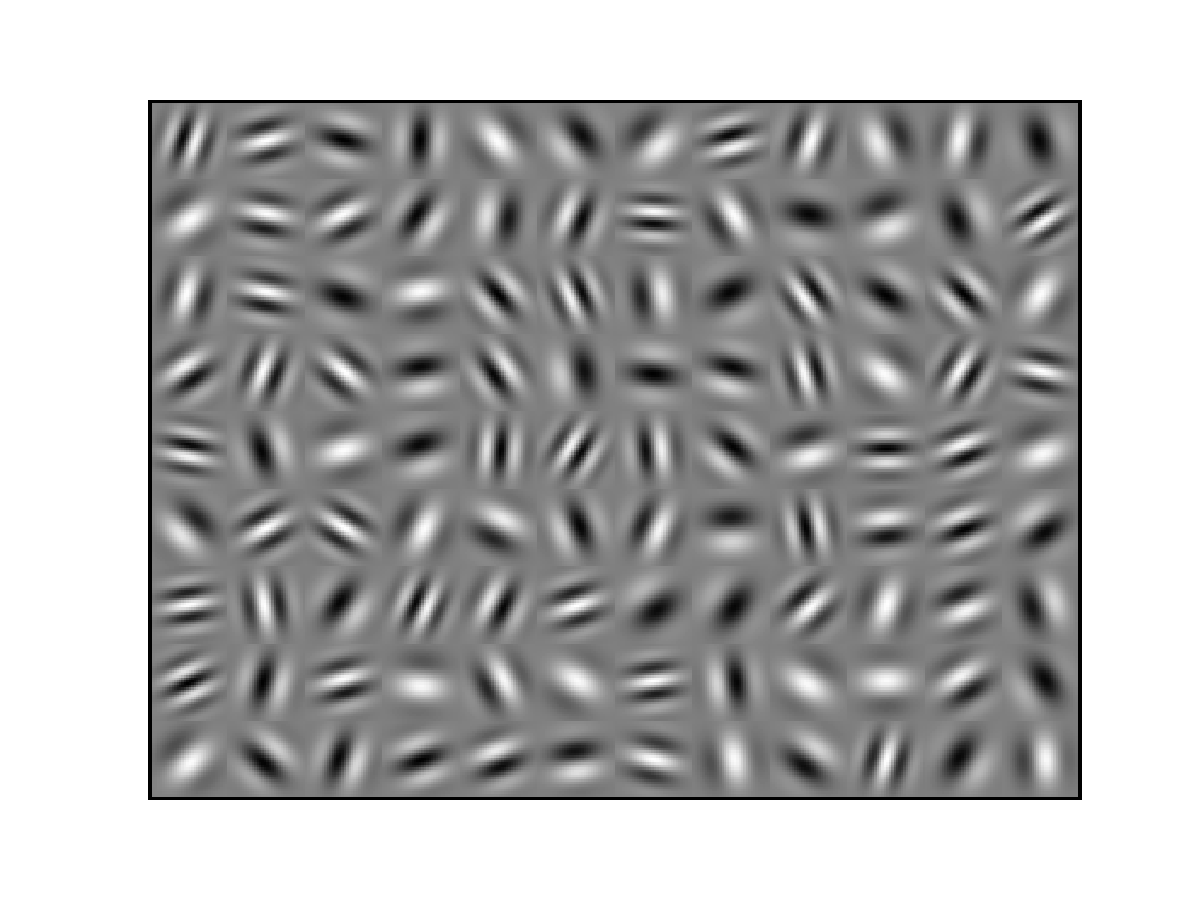
\includegraphics[width=\columnwidth]{gabors.pdf}
  \captionb{A collection of Gabor filters.}{
    Filters vary in frequency, orientation, and phase.
    $\log f \in \mathcal{U}(\log 0.5, \log 1.5)$,
    $\theta \in \mathcal{U}(-\pi, \pi)$,
    $p \in \mathcal{U}(-\pi, \pi)$, $\sigma_u = 0.45$, $\sigma_v = 0.45$.
  }
  \figlabel{gabors}
\end{figure}

\fig{gabors} shows a collection of Gabor filters.
Note that the filters vary in frequency and orientation,
such that each one is suited for detecting edges of a particular width
at a particular orientation.

Gabor filters can be combined with receptive fields,
such that each filter targets a local region of the image.
In fact, this is necessary with Gabor filters,
since edges are local features,
and Gabor filters that cover the whole image will be poorly suited
to detecting them.
It is important to note that the RFs in this case should not be thought of
as a mask, however;
that is, I do not generate full-field Gabor filters,
then use a RF mask to make them local.
Rather, I generate Gabor filters of the desired RF size,
and centre each of these on random points in the image.
Note that the parameters for the Gabor filters are in terms of the coordinates
$x$ and $y$,
which are on the interval $(-1, 1)$
independent of the size of the receptive field.
Changing the receptive field for the Gabor filter encoders
will scale all filters,
thus changing the statistics relative to the image size.


\subsection{Computed Input Weights (CIW)}

\emph{Computed Input Weights} (CIW) is a technique developed by \textcite{Tapson2015}
for generating the input weights (encoders) for a SLFN.
Unlike the previous methods presented here,
which are independent of the training data
(aside from hyperparameters which can be tuned to the data),
this method generates encoders based directly on the training dataset.
Each encoder is chosen as a weighted sum of all the examples
belonging to a particular class,
where weights are randomly chosen from the set of $\{+1, -1\}$.
Thus, each encoder targets a particular class,
but is sensitive only to some examples in that class,
and inversely sensitive to others.
Encoders are chosen to target all the classes in the dataset.
Since the weights on the in-class examples are randomly chosen,
this technique has elements of both random and data-driven encoder generation.

Given $\mat X$, an $M \times D$ matrix of training examples,
where each example belongs to one of $n_c$ classes $c \in C$,
perform the following steps to generate the $N \times D$ encoder matrix $\mat E$:
\begin{enumerate}
  \item For generating the encoders,
    use a normalized version of the training data
    with the mean over all examples and dimensions subtracted out,
    and divided by the standard deviation over all examples and dimensions.
  \item For each class in the dataset, generate $N_c = N / n_c$ encoders,
    using the following procedure:
    \begin{enumerate}
      \item Select $\mat X_c$, an $M_c \times D$ matrix of the set of examples
        that belong to the current class $c$.
      \item Generate a $M_c \times N_c$ random matrix $\mat R_c$
        where each element is either $+1$ or $-1$ with equal probability.
      \item Generate the encoders for the class as $\mat E_c = \mat R_c^T \mat X_c$.
        The full set of encoders $\mat E$ is the concatenation of $\mat E_c$
        for all classes $c \in C$.
    \end{enumerate}
  \item Normalize the encoders $\mat E$ by dividing by each row (each encoder)
    by its $L_2$ (Euclidean) norm.
\end{enumerate}


\subsection{Constrained Difference weights (CD)}

The \emph{Constrained Difference} (CD) algorithm \parencite{Zhu2015}
is another recent technique for generating SLFN encoders
using both data-driven and random elements.
Each encoder is formed as the difference between two training examples
from different classes.
Thus, each encoder tries to separate between two classes.

Given $\mat X$, an $M \times D$ matrix of training examples,
where each example belongs to one of $n_c$ classes $c \in C$,
perform the following steps $N$ times
to generate the $N \times D$ encoder matrix $\mat E$
and bias vector $\vect b$:
\begin{enumerate}
  \item Pick two different classes $a, b \in C$ randomly.
  \item Pick two random examples $\vect x_a$ and $\vect x_b$,
    belonging to the classes $a$ and $b$ respectively.
  \item Let the encoder weight
    $\vect w = 2 (\vect x_a - \vect x_b) / \|\vect x_a - \vect x_b\|_2$,
    and bias $b = (\vect x_a - \vect x_b)^T (\vect x_a + \vect x_b) / \|\vect x_a - \vect x_b\|_2$.
\end{enumerate}


\section{Decoding methods}
\scnlabel{nef-decoding}

Another key question with fixed-encoding methods
is how to find decoding weights.

At the core of this question is the choice of loss function,
which defines the objective that we wish to minimize
(see \scn{objective-functions} for an overview of loss functions).
For classification, we ultimately wish to minimize the classification error,
that is, the number of examples incorrectly classified.
However, the classification error is a discrete value,
prohibiting us from using it directly \parencite{Toh2008}.
For example, if we make a small change to our model,
it may not change how any example in our training set is classified,
and thus the classification error does not change.
Yet, we need to know whether this change is an improvement or not;
it may move some incorrectly classified examples
closer to being correctly classified,
and many changes in that same direction may lead to better classification error.
The idea behind loss functions for classification
is to find a continuous value---the loss---%
which when minimized will also minimize the classification error.

Many classification loss functions were originally formulated
for binary classification, where we have only two output classes.
In object classification, there are typically many different classes,
since there are many types of objects in the world.
Thus, we are interested in loss functions
for multiclass classification,
where we have more than two classes.

I focus on loss functions that result in a linear classifier.
Given an $M \times N$ matrix of hidden node activations $\mat A$
(found by applying the encoders and neural nonlinearity to the training data points),
we wish to find an $N \times C$ matrix of decoding weights $\Dec$
that map the hidden neuron activations to outputs $\mat Y$:
\begin{align}
  \mat Y = \mat A \Dec \text{ .}
\end{align}
$\vect y_k$ represents one row of $\mat Y$,
that is, the output of the system for training example $k$;
$\dec_i$ represents one column of $\Dec$,
that is, the decoders for one of the $C$ output dimensions.
In training this classifier we use either the vector of labels $\vect l$
for the $M$ training examples,
or the equivalent one-hot representations $\mat T$,
an $M \times C$ matrix where
\begin{align}
  T_{ki} = \begin{cases}
    1 & \text{if } i = c(k) \\
    0 & \text{otherwise}
  \end{cases} \text{ ,}
\end{align}
$c(k)$ is the correct class (label) for example $k$,
and $\vect t_k$ is one row of this matrix (\ie/ the one-hot encoding of example $k$).

My main reason for using a linear classifier
is that it can be directly mapped onto neural connection weights.
Note that this does not mean we are limited to linear optimization methods;
two of the loss functions examined here (softmax loss and hinge loss)
require nonlinear optimization,
yet result in a linear classifier.
Also, when used as part of a larger neural system,
the classifier may connect directly into nonlinear components,
such that the entire system forms a type of nonlinear classifier.
For example, the classifier may connect into a system like
the basal ganglia,
which chooses the maximum output of the classifier
and routes information accordingly.

Loss functions have been explored extensively
in machine learning \parencite[\eg/][]{Rosasco2004},
and it is known that squared loss
is not optimal for classification \parencite[][p. 186]{Bishop2006}.
Yet, these loss functions are typically not used in the ELM literature
\parencite[\eg/][]{McDonnell2015}.
A notable exception is the work of \textcite{Toh2008},
who introduces weighted squared loss for ELMs.
This section explores loss functions in the context of SLFNs,
to bring more awareness of the benefits of alternative loss functions
to researchers working with SLFNs and other fixed-encoding networks.


\subsection{Squared loss}
\scnlabel{squaredloss}

Squared loss, also known as the least-squares technique,
is common for solving regression problems.
It minimizes the sum of squared errors between each predicted point
and the corresponding target point.
%% Squared loss generalizes least squares to classification problems.
In the multiclass case it uses a one-hot encoding of the target class $\mat T$
as the target point.

The squared loss across all $M$ examples is given by
\begin{align}
  %% O_\text{MSE} = \frac{1}{N} \sum^N_k \sum_i (y^{(k)}_i - y^{*(k)}_i)^2.
  %% O_\text{MSE} = \frac{1}{M} \sum^M_k \|\vect y_k - y^*_k\|_2^2.
  O_\text{squared} = \sum^M_k \|\vect y_k - \vect t_k\|_2^2 \text{ .}
  \eqnlabel{squaredloss}
\end{align}
This amounts to training a one-vs-all classifier for each class.
We wish to find the linear decoders $\Dec$,
a matrix mapping the $N$ hidden neuron activities to the $C$ categories.
The solution to this problem, in matrix form, is
\begin{align}
  \Dec = (\mat A^T \mat A)^{-1} \mat A^T \mat T.
  \eqnlabel{lstsq}
\end{align}
This is found by taking the derivative of \eqn{squaredloss}
and setting it equal to zero to find the stationary points.
Because the objective function is quadratic,
the single stationary point is necessarily a minimum.

Squared loss is not ideal for classification,
since it leads to slower convergence than softmax loss and hinge loss
\parencite{Rosasco2004},
and often results in sub-optimal classification boundaries \parencite[][p. 187]{Bishop2006}.
Part of the reason for this is that it penalizes outliers heavily,
such that larger errors are much more costly than smaller ones \parencite[\eg/][p. 186]{Bishop2006}.
For example, consider a classifier that has two outputs,
corresponding to two different classes.
Say we have two examples that are both labeled as the first class:
their one-hot target vectors will both be $\vect y^* = [1, 0]$.
If the classifier outputs $y_1 = [1, 0.9]$ for the first example,
it has correctly classified it
by a margin of 0.1 (the difference between the correct category output
and the next highest output).
The loss on this example is $\|y_1 - y^*\|_2^2 = (0.9)^2 = 0.81$.
Say for the other example (of the same category),
the classifier outputs $y_2 = [0.4, 0.6]$.
It has incorrectly classified this example by a margin of 0.2.
The loss on this example is $\|y_1 - y^*\|_2^2 = (-0.6)^2 + (0.6)^2 = 0.72$.
Therefore, the classifier does better on the first example,
but the loss is lower on the second example.
This is the opposite of what we want!

Another related problem becomes apparent as we move to more classes.
This problem is that the loss function over-penalizes when
there are multiple competing classes.
Consider a classifier that has three outputs;
again, we look at two examples from the first class,
thus with one-hot target vector $\vect y^* = [1, 0, 0]$.
If the output for the first example is $y_1 = [1, 0.8, 0.8]$,
and for the second example is $y_2 = [0.8, 1, 0]$,
the loss for the first example is $2 (0.8)^2 = 1.28$
and for the second example $(-0.2)^2 + (1)^2 = 1.04$.
The first example is correctly classified by a margin of 0.2,
whereas the second is incorrectly classified by a margin of 0.2,
but the second example has the smaller loss.
The difference between the two examples is that
the first has significant errors in two outputs (outputs two and three),
whereas the second only has a significant error in the second output.
The loss function penalizes the case where many classes have significant errors,
even though this is often not a problem as long as the correct class
is beating all other classes by a significant margin.

These problems both occur because the classifier is treating each element
of the target vector as an independent regression variable.
To achieve better results
requires some sort of dependence
between the outputs for these regression variables.


\subsection{Weighted squared loss}
\scnlabel{wsquaredloss}

To address the problem that linear least squares
over-penalizes multiple competing classes,
I investigated weighting errors on examples of the target class (positive examples)
more heavily than those of other classes (negative examples).
If we view each output dimension of the classifier
as an independent one-vs-all classifier---%
which is how linear least squares treats the problem---%
then it is intuitive that for each one-vs-all classifier,
we want a balance between positive and negative examples.
Re-weighting the examples achieves this balance.

\textcite{Toh2008} came to a similar conclusion,
from a more theoretical basis.
They derived the same weighted least squares solution
by approximating the discontinuous classification error as best possible
with a quadratic function.
Despite this significant result,
many modern SLFNs still use unweighted linear least squares \parencite{McDonnell2015}.

Weighted least squares is a popular variant of least squares
whereby different residuals can be given different weights.
If there is measurement uncertainty (error)
associated with each of the regression points,
and this uncertainty varies between points and can be quantified,
weighted least squares allows one to account for this uncertainty \parencite{Fieguth2010}.

Linear weighted least squares is defined by a similar objective function
to ordinary linear least squares (\eqn{squaredloss}),
except with scalar weights $w_k$ on each error:
\begin{align}
  \left[O_\text{w-squared}\right]_i = \sum^M_k w_k (Y_{ki} - T_{ki})^2.
  \eqnlabel{wsquaredloss}
\end{align}
It is defined here for the one-dimensional case (\ie/ for output dimension $i$),
to allow for separate weights for each dimension of the output,
based on whether that dimension represents the correct or incorrect class
for each example (see below).
%% \begin{align}
%%   \vect x = \argmin_x \sum_k w_k r_k^2
%%   \text{, where } r_k = A_k \vect x - y_k
%%   \eqnlabel{wlstsq-obj}
%% \end{align}
%% for the one-dimensional case.

Taking the derivative and setting it equal to zero, as before, we find that:
\begin{align}
  \Dec = (\mat A^T \mat W \mat A)^{-1} \mat A^T \mat W \vect T_{\cdot i}
\end{align}
where $\mat W$ is a square diagonal matrix of the weights $w_k$
and $\vect T_{\cdot i}$ is column $i$ of $\mat T$.
This system can be solved using the same solution as for unweighted least squares,
including SVD if the system is ill-conditioned,
and Cholesky decomposition if it is well-conditioned.

We can weight examples based on their frequency,
such that the (typically less frequent) positive examples
receive the same total weight as the negative examples:
\begin{align}
  n^+ w^+ = n^- w^-
\end{align}
where $n^+$ and $n^-$ are the numbers of positive and negative examples,
and $w^+$ and $w^-$ are the weights on the positive and negative examples.
We also wish the total weight to sum to the number of examples:
\begin{align}
  n^+ w^+ + n^- w^- = n^+ + n^- \text{ .}
\end{align}
This results in weights
\begin{align}
  w^+ &= \frac{1}{2p^+} \\
  w^- &= \frac{1}{2(1 - p^+)}
\end{align}
where $p^+ \equiv n^+ / (n^+ + n^-)$ is the fraction of positive examples.
If both categories appear equally frequently (\ie/ $p^+ = 0.5$),
then $w^+ = w^- = 1$,
and the method is equivalent to unweighted least squares.

The key to this method is that this weighting is different
for each one-vs-all classifier,
such that each one requires solving a different linear system.
Specifically,
in the case of unweighted least squares,
we can solve
%% $\Dec = (\mat A^T \mat A + \lambda \mat I)^{-1} \mat A^T \mat T$
$\Dec = (\mat A^T \mat A)^{-1} \mat A^T \mat T$
simultaneously for all columns of $\mat T$.
With weighted least squares method we must solve
\begin{align}
  %% \Dec_{\cdot,i} = (\mat A^T \mat W_i \mat A + \lambda \mat I)^{-1} \mat A^T \mat W_k \mat T_{\cdot,i}
  \Dec_{\cdot,i} = (\mat A^T \mat W_i \mat A)^{-1} \mat A^T \mat W_k \mat T_{\cdot,i}
\end{align}
where $\Dec_{\cdot,i}$ and $\mat T_{\cdot,i}$ are the $i$\sth/ columns of $\Dec$ and $\mat T$,
and $\mat W_i$ is a unique set of weights for each value of $i$.
Luckily, structure in the weights allows us to solve these systems
with the same order of computation
as solving the unweighted least squares system (see \app{wlls}).


\subsection{Softmax loss}
\scnlabel{softmaxloss}

The softmax loss (also known as the logistic loss or cross-entropy loss)
allows us to better model the max function that our classifier output
passes through when determining the classification error.
In the multiclass case,
we pass the linear classifier output through the softmax function,
which normalizes the outputs relative to one another.
The softmax function is so named because it is a
differentiable (``soft'') version of the max function.

The softmax loss is given by
\begin{align}
  O_\text{log} &= -\sum_k^M \left[\log (\vect\sigma(\vect y_k))\right]_{c(k)}
\end{align}
where $c(k)$ is the label index of the $k$\sth/ example,
and $\vect\sigma$ is the softmax function
\begin{align}
  \vect\sigma(\vect y) = \frac{e^{\vect y}}{\sum_i e^{y_i}} \text{ .}
\end{align}
The derivative of the softmax loss function is surprisingly simple:
It is simply the error difference between the output of the softmax function
and the target one-hot representation:
\begin{align}
  \diff{O_\text{log}}{\vect y_k} &= \vect\sigma(\vect y_k) - \vect t_k \\
  \diff{O_\text{log}}{\Dec} &= \mat A^T \diff{O_\text{log}}{\mat Y} \text{ .}
\end{align}
Despite the simplicity of this derivative,
it is still nonlinear, due to the softmax function.
Therefore, we have to solve using nonlinear optimization techniques.
The L-BFGS method \parencite{Liu1989} works quite well.\footnote{
  Using the implementation in Scipy: \url{http://www.scipy.org}}

The softmax loss is closely related to the classification error.
If an example is correctly classified,
then the softmax loss is necessarily lower on that example
than if it is incorrectly classified.
That is, the softmax loss can never be higher for a correctly classified example
than for an incorrectly classified one.
Compare this with squared loss,
which we saw by example in the previous section could have lower loss
for incorrectly classified examples than for correctly classified ones.
This does not mean, however, that minimizing the softmax loss
will necessarily result in the best possible linear classifier.
For example, if one example is misclassified by the classifier by a huge margin,
resulting in a huge loss,
this could be a higher total loss than a number of examples
that are only misclassified by a small margin.
Such a situation can happen with outliers,
where one training example looks very different than other members of its class,
or with incorrectly labeled data (\ie/ noisy labels).
Thus, even with softmax loss,
the lowest loss does not result in the lowest training-set classification error.
However, the relationship between loss and classification error
is much closer than with squared loss.


\subsection{Hinge loss}
\scnlabel{hingeloss}

Hinge loss maximizes the margins between the correct class and incorrect class
for all the training examples,
with a maximum margin at which we consider two examples perfectly distinguished.
This is the loss traditionally associated with support vector machines.
%% That is, in the binary classification situation,
%% we want the margin between the co

There is no unique way to generalize hinge loss to the multiclass problem.
One choice is to maximize the margin of the correct class
over the next highest class \parencite{Crammer2001}.\footnote{
  This is the formulation used here.
  A comparison of formulations of hinge loss is beyond the scope of this thesis.}
For example $k$, the margin $m_k$ is given by:
\begin{align}
  m_k = Y_{kc} - \max_{i \ne c} Y_{ki}
\end{align}
where $c$ is the correct class for example $k$,
$Y_{kc}$ is the classifier output for the correct class,
and $Y_{ki}$ is the classifier output for one of the incorrect classes $i$.
Of course, this margin can be negative if the correct class $c$
does not have the highest response
(in which case the classifier is incorrectly classifying example $k$).
Our objective function is
\begin{align}
  O_\text{hinge} = \sum_k \max\left(0, 1 - m_k\right) \text{ .}
\end{align}
Any example that has a margin $\ge 1$ is considered ideally classified,
and has zero loss.
The loss for all other examples is one minus the margin.

The derivative of this hinge loss with respect to the classifier output is
\begin{align}
  \diff{O_\text{hinge}}{Y_{ki}} = \begin{cases}
    -1 & \text{if } i = c \\
    1 & \text{if } i = a \\
    0 & \text{otherwise}
  \end{cases}
\end{align}
That is, increasing $Y_{kc}$ will decrease the loss,
and increasing $Y_{ka}$ will increase the loss,
where $a = \argmax_{i \ne c} Y_{ki}$ is the highest response not of the correct class.
We can then find the derivative with respect to the classifier weights
by using the chain rule:
\begin{align}
  \diff{O_\text{hinge}}{\Dec} &= \mat A^T \diff{O_\text{hinge}}{\mat Y} \text{ .}
\end{align}

One important aspect of the hinge loss is that it is
very dependent on the magnitude of the classifier outputs $\mat Y$,
and by extension the decoding weights $\Dec$.
For example, if the classifier has many examples correct by a given margin,
doubling the classifier weights will double that margin for all correct examples.
For this reason, most support vector machines that use hinge loss
also use a constraint on the magnitude of the weight vector,
typically an equality constraint ensuring it has a norm of one.
I have not employed such a constraint,
but rather used regularization on the weight magnitude
to a similar effect (see \scn{dec-regularization}).
Though other loss functions (\eg/ softmax loss)
can also be vulnerable to situations where larger magnitudes yield lower loss,
this effect seems the most prominent with hinge loss (see \fig{nef-regularization}),
and thus regularization is particularly important with this loss function.

Like the softmax loss,
the hinge loss function has the benefit
that it is closely related to the classification error.
If an example is correctly classified,
then the hinge loss for that example is necessarily lower
than if the example is incorrectly classified.
This makes it a better loss function than the squared loss.

% Lee2004?? I put this here before, but I can't remember why


\subsection{Weight norm regularization}
\scnlabel{dec-regularization}

Adding a cost on the magnitude of the weights
can both help with overfitting,
and can help reduce noise when using spiking neurons \parencite{Eliasmith2003}.
This is not a cost or loss function by itself,
but rather a term that can be added to any other loss function.

Given an objective function $O$,
we can create a regularized version $O_\text{reg}$:
\begin{align}
  O_\text{reg} = O + \lambda \|\Gamma \Dec\|_p
\end{align}
where $\Dec$ is the set of parameters (weights) being learned.
Thus, we are taking the $L_p$ norm on a linear projection $\Gamma$ of our weights.
Often, we take $\Gamma$ to be a scalar multiple of the identity matrix,
such that we are simply minimizing the norm of the weights themselves.

If we also take the norm to be the $L_2$ (Euclidean) norm,
we get \emph{ridge regression}:
\begin{align}
  O_2 = O + \frac{\lambda}{2} \|\Dec\|_2^2.
\end{align}
This penalizes the sum of squared elements of $\Dec$.
It is particularly useful when combined with linear least squares,
since its derivative is also linear, thus still allowing a linear solution.

If we instead take the norm to be the $L_1$ (Manhattan) norm,
we get the \emph{lasso}:
\begin{align}
  O_1 = O + \lambda \|\Dec\|_1.
\end{align}
This results in sparse $\Dec$, where many elements are zero.

Here, I focus on $L_2$ norm regularization,
mainly because it can be used with squared loss functions
and still allow analytic solutions
(thus accelerating the decoder-finding process).
The $L_2$ norm was also used by \textcite{Eliasmith2003}
to reduce the amount of variance from spikes in the output of a spiking network,
and thus has benefits specific to spiking networks.

The effect that regularization will have depends on
the scale of the activity matrix $\mat A$.
Because I have written my loss functions as taking
the sum of the losses on all points, rather than the mean,
the effect of regularization also depends on the number of points $M$.
Thus, I scale the regularization constant $\rho$
by both the maximum activity $\|\mat A\|_\infty$ and by $M$,
to yield the total regularization parameter $\lambda$:
\begin{align}
  \sigma &= \rho \|\mat A\|_\infty \\
  \lambda &= M \sigma^2
\end{align}
By squaring $\sigma$, this equation is tuned for use with an $L_2$ norm.
%% Determining the regularization constant for an $L_1$ norm

% introduce LOO cross-validation, either here or maybe in intro? Probably in intro
Determining the regularization parameter $\rho$ is not trivial.
Cross-validation techniques estimate the generalization error of a method on a dataset;
by applying the cross-validation technique for many different $\rho$ values,
one can determine a near-optimal choice for $\rho$.
Leave-one-out (LOO) cross-validation computes the classifier on all data points
except one, then computes the classification error on the excluded data point.
Repeating this for all data points yields a robust estimate of the generalization error.
Unfortunately, it scales linearly with the number of training data points,
making it very costly for our application (where solving for the classifier is costly).
Other possible cross-validation methods include using a number of randomly-selected
subsets from the dataset for each $\rho$ value,
or taking a single subset of the training data and holding it aside as a validation set.

% talk about Rifkin2007 method
\textcite{Rifkin2007} demonstrated that the regularization parameter
can be found using leave-one-out (LOO) cross-validation
at little extra cost when using direct least-squares solution methods.
They derived an expression for the LOO error
that depends only on the eigendecomposition of
the covariance matrix ($\mat A^T \mat A$) of the system
(they also derive the same result using the singular value decomposition of $\mat A$).
Using this method, the effect of different values of $\rho$ on the LOO error
to be tested without re-solving the system itself,
and a good value for the regularization parameter
can be found at (theoretically) little extra cost.

The core of the method is the fact that for a linear least-squares problem,
as formulated in \eqn{lstsq} (with regularization),
the vector of LOO errors $\vect e_\text{LOO}$
for each training sample is given by
\begin{align}
  \vect e_\text{LOO} = \frac{
    \mat Y - \mat A (\mat A^T \mat A + \lambda\mat I)^{-1} \mat A^T \mat Y}{
    \diag(I - \mat A (\mat A^T \mat A + \lambda\mat I)^{-1} \mat A^T)}
  \eqnlabel{rifkin}
\end{align}
where $\diag(\mat X)$ is the vector of diagonal elements of matrix $\mat X$,
and the division is performed elementwise.
The covariance matrix can be factored using an eigendecomposition,
\ie/ $\mat A^T \mat A = \mat Q \Lambda \mat Q^T$,
where $\mat Q$ is an orthogonal matrix and $\Lambda$ is a diagonal matrix.
Thus, $(\mat A^T \mat A + \lambda\mat I)^{-1} = \mat Q (\Lambda + \lambda)^{-1} \mat Q^T$.
This allows us to re-write \eqn{rifkin} as
\begin{align}
  \vect e_\text{LOO} &= \frac{
    \mat Y - \mat A \mat Q (\Lambda + \lambda\mat I)^{-1} \mat Q^T \mat A^T \mat Y}{
    \diag(I - \mat A \mat Q (\Lambda + \lambda\mat I)^{-1} \mat Q^T \mat A^T)}
  \eqnlabel{rifkin-eigen} \\
  &= \frac{
    \mat Y - \mat P (\Lambda + \lambda\mat I)^{-1} \mat P^T \mat Y}{
    \diag(I - \mat P (\Lambda + \lambda\mat I)^{-1} \mat P^T)}
\end{align}
where $\mat P = \mat A \mat Q$.
The denominator $\vect d$ of this expression can be calculated efficiently as
\begin{align}
  d_i = \sum_j^N \frac{P_{ij} P_{ij}}{\Lambda_{jj} + \lambda}.
\end{align}
Unfortunately, this computation still involves computing the matrix product
$\mat P = \mat A \mat Q$, which is $O(MN^2)$.
Using the form of \eqn{rifkin-eigen} is no better:
while the numerator can be computed
as four successive $O(MNC)$ products with the matrix $\mat Y$,
the denominator involves an unavoidable $O(MN^2)$ matrix-matrix product,
which is more expensive since $C \ll N$.
Furthermore, when using this method with the weighted squared loss,
we need to form $\mat P$ again for each weighting,
since the weighting affects the value of $\mat Q$.
Thus, the cost of this method is $O(CMN^2)$ for weighted least squares.
Unfortunately, this method only works for squared loss functions,
and does not generalize to softmax loss or hinge loss.


\section{Spiking methods}
\scnlabel{nef-spiking-methods}

Simulating a network with spiking neurons
is different than running an ANN with rate neurons.
Spiking neurons are dynamic and must be run \emph{online},
with each stimulus (image) presented for a period of time
such that the spiking neurons have time to respond with a spike train signal.
ANNs---on the other hand---are almost always run offline,
presenting as many images to the network at a time as desired,
and responses for all images generated with a single forward pass
through the network.\footnote{
  This assumes the networks are fully feedforward,
  as are all the networks presented and discussed in this thesis.
  Recurrent networks require presenting inputs over a span of time.}
This change from offline to online introduces a number of new design decisions.

One of the most important design decisions
is how the classification is performed.
In biological systems, when we examine the macro-level behaviour of the system,
we are always looking at the full system,
from the external stimulus (image) to the physical response
(motor movement or speech).
The network presented here does not include a motor system
to close this behaviour loop,
so when we evaluate it based on its output,
we do not get the full picture of how it would operate
in a closed-loop system.

For the evaluation of the spiking networks in this thesis,
the category selected by the classifier
is the category with the maximum average response
during the presentation of each stimulus.
The advantages of this approach are that it is simple,
it captures how the system would perform on a neuromorphic chip,
and it allows for a fair comparison with current machine-learning approaches.
The main disadvantage is that selecting the maximum of a number of values
is not a function that can be computed perfectly or easily in neurons,
particularly when there are multiple values near the maximum.
The Spaun brain model \parencite{Eliasmith2012}
uses a detailed model of the basal ganglia to compute this operation.
Such a basal ganglia model could be included
as part of the networks presented here,
to get a better idea of how they might function as part of an end-to-end system.

There are three new hyperparameters associated with running our network online
in spiking neurons, that do not appear in the offline network:
\begin{enumerate}
  \item The presentation time $t_p$ that each stimulus is shown for,
  \item the classification start time $t_c$,
    which determines how long after the stimulus is first presented
    the averaging for classification starts, and
  \item the time constants $\taus$ of any synapses in the network.
\end{enumerate}
In terms of accuracy, a longer presentation time is always better,
since it allows more time for any transient dynamics in the network to settle
and for the output to average across a larger time window,
thus reducing some of the variability associated with spiking neurons.
In practice, choosing the presentation time
is always a tradeoff between accuracy and throughput,
where shorter presentation times allow more stimuli to be classified
per unit time,
at the cost of accuracy.

The classification start time determines at what point after each stimulus is shown
do we begin averaging the network outputs for classification.
This allows the classifier to ignore the initial transient output of the network.
It is important because I test these networks continuously
over the whole series of test inputs,
preserving the network state from one input to the next.
Some other works \parencite[\eg/][]{Cao2014,Diehl2015} present each stimulus separately,
resetting the state of the network between presentations;
in that setup, there is no transient state from previous presentations,
so using the whole presentation time for classification is not problematic.

Finally, the synapse time constants determine the amount of filtering
applied to the output of each neuron.
For the networks in this chapter,
which only have a single hidden layer,
then this is equivalent to filtering on the output (since the classifier is linear).
For the deep networks examined in later chapters,
the filtering is applied to the output of \emph{each} neuron layer.
All networks in this thesis use alpha synapses (\eqn{alpha-synapse}).
The time constants of the synapses affect the amount of time required
for information to propagate through the network,
and thus the value of the time constant (combined with the network depth)
should be the main factor determining the choice
of the classification start time $t_c$.

For the networks in this chapter,
I chose $t_p = 70$ ms, $t_c = 5$ ms, and $\taus = 0$ ms.
This allows sufficient time to classify each input accurately
while still allowing the network to process images quickly.
Since the networks only have a single hidden layer
and the classification method already averages over their output,
I found that synaptic filtering was unnecessary.

All simulations were performed using the Nengo neural simulator \parencite{Bekolay2014}.


%%%%%%%%%%%%%%%%%%%%%%%%%%%%%%%%%%%%%%%%%%%%%%%%%%%%%%%%%%%%%%%%%%%%%%%%%%%%%%%%
\section{Results}

To assess the performance of the encoding and decoding methods
described in this chapter,
I used the MNIST dataset as a benchmark.


\subsection{Encoding}
\scnlabel{enc-results}

\begin{figure}
  \centering
  \newcommand{\gwidth}{0.45\columnwidth}
  \begin{tabular}{cc}
    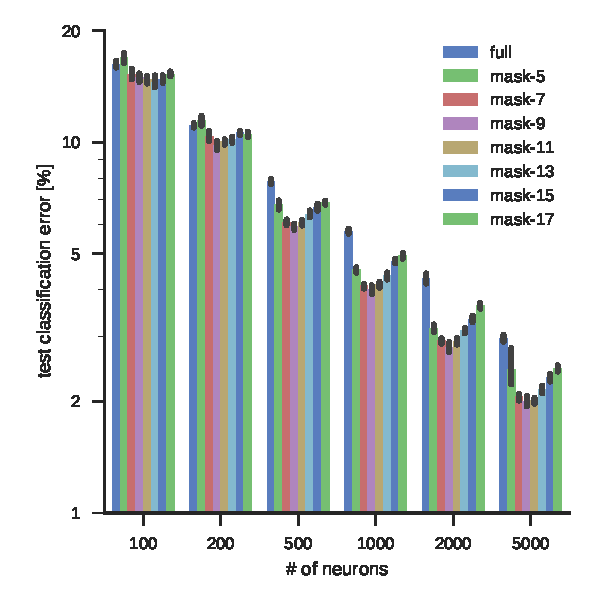
\includegraphics[width=\gwidth,clip=true,trim=3mm 3mm 3mm 3mm]{mnist_compare_encoders_masks.pdf} &
    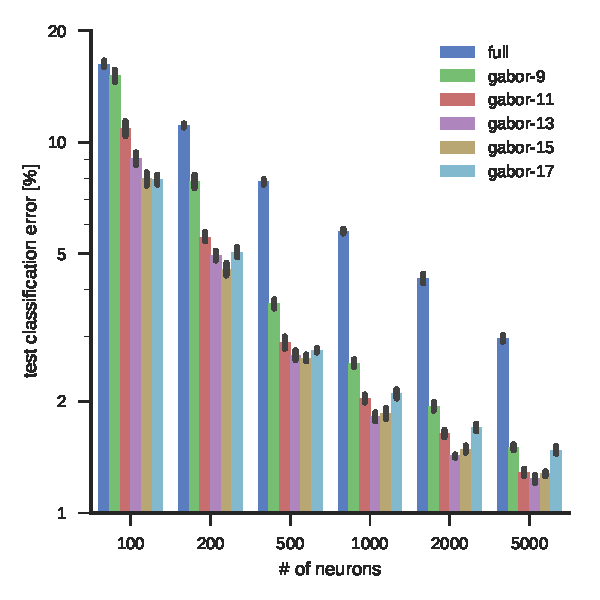
\includegraphics[width=\gwidth,clip=true,trim=3mm 3mm 3mm 3mm]{mnist_compare_encoders_gabors.pdf} \\
    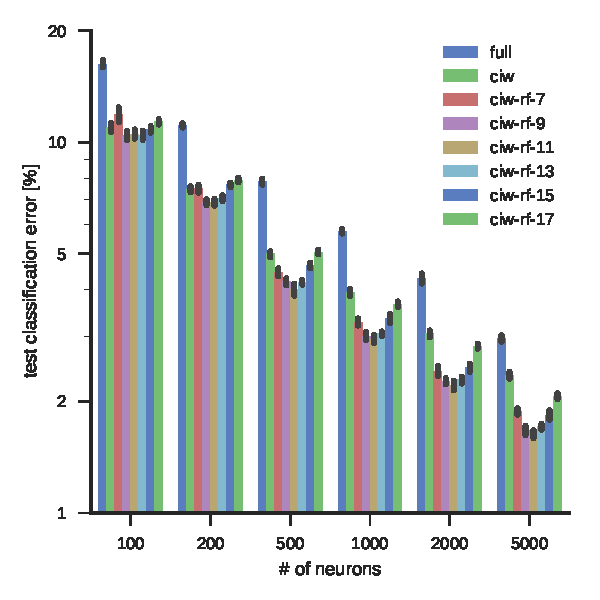
\includegraphics[width=\gwidth,clip=true,trim=3mm 3mm 3mm 3mm]{mnist_compare_encoders_ciw.pdf} &
    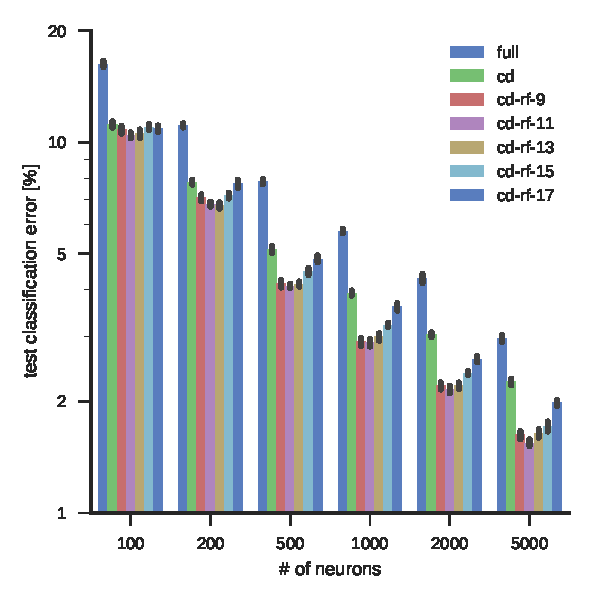
\includegraphics[width=\gwidth,clip=true,trim=3mm 3mm 3mm 3mm]{mnist_compare_encoders_cd.pdf} \\
  \end{tabular}
  \captionb{Different choices of encoders for SLFNs.}{
    \textbf{Top left:} Using limited receptive fields (``mask-\#'') reduces
    test-set error vs fully-connected random encoders (``full'').
    RFs around the $9 \times 9$ size perform the best.
    \textbf{Top right:} Using Gabor filters with varying sizes of RFs (``gabor-\#'')
    also reduces test-set error, with $13 \times 13$ RF size working best.
    The Gabor filter parameters are:
    $f \in \mathcal{U}(0.2, 2.0)$,
    $\theta \in \mathcal{U}(-\pi, \pi)$,
    $p \in \mathcal{U}(-\pi, \pi)$, $\sigma_u = 0.45$, $\sigma_v = 0.45$.
    \textbf{Bottom left:} CIW encoders also improve performance,
    with a $11 \times 11$ RF size working best.
    \textbf{Bottom right:} CD encoders also follow the trend,
    again with $11 \times 11$ RF size working best.
    %% \# indicates the receptive field size.
  }
  \figlabel{nef-encoder-choices}
\end{figure}

\fig{nef-encoder-choices} shows detailed results
for each of the four methods examined.
In the figure, ``full'' refers to fully connected,
independent and identically distributed (i.i.d.) random encoders,
which generally perform the worst.
Adding a receptive field (RF) mask to i.i.d. random encoders (``mask-\#''),
such that each encoder is only connected to a limited local region of the image,
improves performance.
There are some receptive field sizes, such as $3 \times 3$ (not shown),
for which the RF i.i.d. encoders perform worse than fully connected ones.
Other, non-i.i.d. methods of generating encoders can be combined
with receptive fields to improve performance.
With Gabor filters, using a RF size of $13 \times 13$ works best.
Full-field Gabor filters perform poorly (not shown),
because edges are local features,
and thus filters for detecting them must also be local.
Finally, the RF method can be combined with the CIW and CD methods
to improve their performance;
this supports the results of \textcite{McDonnell2015}.


\begin{figure}
  \centering
  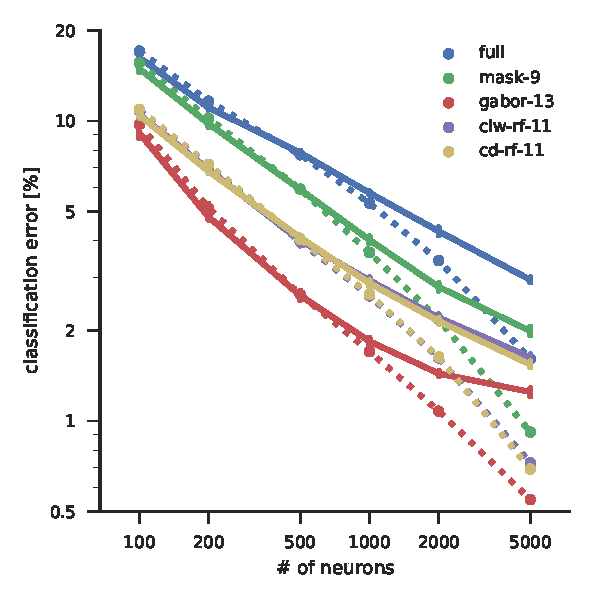
\includegraphics[width=4in]{mnist_compare_encoders_besttt.pdf}
  \captionb{Encoder choices for SLFNs with optimal RF size.}{
    Training-set error (dotted line) and test-set error (solid line)
    for the five encoding methods,
    using the optimal RF sizes as determined by \fig{nef-encoder-choices}.
    The number in each label indicates the RF size.
  }
  \figlabel{nef-encoder-summary}
\end{figure}

\fig{nef-encoder-summary} shows the result of testing a number of different methods
of choosing encoders.
Encoder choice has a significant effect on test error rates.
Using i.i.d. encoders with limited receptive fields (RFs),
results in significantly better performance than fully connected i.i.d. encoders,
if the size of the RFs is chosen well.
The data-driven CIW and CD methods again offer some improvement,
though surprisingly it is the Gabor filter encoders that perform the best.

It is not surprising that Gabor filters perform better
than the i.i.d. methods.
Gabor filters are good at sparsely representing natural images \parencite{Olshausen1996},
and most deep networks that perform well on real-world object classification tasks
have been found to have something like Gabor filters in the first layer \parencite[\eg/][]{Krizhevsky2012}.
These results show that the Gabor filters do not have to be
individually tuned to the data;
a wide range of filters covering the frequencies and orientations
observed in the input data
is able to achieve high levels of accuracy on MNIST.
It is surprising is that Gabor filter encoders
outperform the CIW and CD methods,
despite the latter being tuned specifically to the MNIST dataset.

The optimal size of receptive field (RF) varied depending on whether the
encoders were i.i.d. or Gabor filters.
Larger RFs worked better with Gabor filters.
This could be because Gabor filters already have a windowing aspect to them,
since they are multiplied spatially by a Gaussian amplitude function.
This creates an effective RF for the Gabor filters that is
smaller than the full RF of the filters;
that is, the pixels at the edges of the filters have low weights,
and have little effect on the filter response.
The effective RF for the Gabor filters is thus closer
to the optimal i.i.d. RF
than the full RF of the Gabor filters indicates.
An additional factor is that the frequency range of the Gabor filters
was not optimized in any rigorous way.
Since the frequencies are set relative to the RF size,
varying the RF size varies the frequency spectrum of the filters.
Thus, the optimality of the $13 \times 13$ Gabor filters
might also have to do with the frequency content of those filters.



\subsection{Decoding}
\scnlabel{dec-results}

\begin{figure}
  \centering
  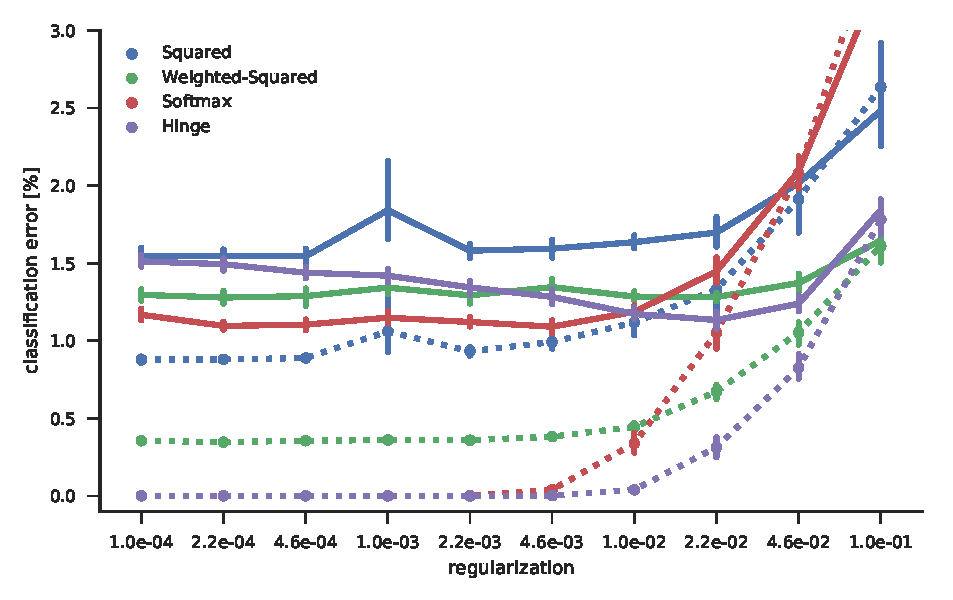
\includegraphics[width=\columnwidth]{mnist_compare_decoder_regularization.pdf}
  \captionb{Effects of regularization on different loss functions.}{
    Dotted and solid traces show training- and test-set classification errors,
    respectively.
    Some loss functions---namely squared loss and weighted squared loss---%
    show best test-set performance when regularization is negligible.
    Other loss functions---namely softmax loss and hinge loss---show
    best test-set performance for nonzero, moderate amounts of regularization.
    Error bars on test-set results show 95\% confidence intervals
    of the mean classification error across 10 trials.
  }
  \figlabel{nef-regularization}
\end{figure}

The amount of regularization has a significant effect on decoding accuracy,
such that comparing different loss functions is only informative
if the amount of regularization is also accounted for.
\fig{nef-regularization} shows the effects of the amount of regularization
on both the training- and test-set classification errors
for different loss functions.
As the figure shows,
some loss functions (least-squares and weighted least-squares)
are optimal with no regularization.
Adding regularization in small amounts has no affect on performance,
and large amounts of regularization decrease performance.
For other loss functions (softmax and hinge loss),
a moderate amount of regularization results in the best performance.
This is most evident with hinge loss,
because with hinge loss it is very easy to increase the margins
on the training data simply by increasing the magnitude of the weights,
without helping with generalization, as discussed in \scn{hingeloss}.
The reason that hinge loss and softmax
benefit from moderate amounts of regularization
is possibly because they are also the most powerful loss functions.
As shown in \fig{nef-regularization},
these loss functions are able to completely fit the training data,
achieving zero loss with low levels of regularization.
Adding regularization helps to reduce this overfitting,
leading to better generalization.

The optimal amounts of regularization for softmax loss ($\sim 4.6\times10^{-3}$)
and hinge loss ($\sim 2.2\times10^{-2}$) are quite different.
This is because these loss functions use different units.
Hinge loss is based on the margin of the correct output over the next highest output,
thus it is in the same units as the linear classifier output.
Softmax loss is the negative log probability of the correct output
after being passed through a softmax function.
Taking the log of a softmax function output
does result in a value in the same units as the linear classifier output,
but normalized by the log of the sum of all exponentiated outputs.
The result is that softmax loss has a significantly different magnitude
than the corresponding hinge loss;
the optimal amount of regularization will vary accordingly.

%% Hinge loss is shows the most variation between the
%% unregularized ($\sim$1.5\% test error) and
%% regularized ($\sim$1.1\% test error) variants.
%% This may be because the hinge loss margin depends on
%% the magnitude of the output weights.
%% Thus, even if the angle of the hyperplane defined by the output weights is not optimal,
%% a larger margin may be achievable simply by increasing the weight magnitude.
%% Applying regularization penalizes the weight magnitude,
%% forcing the optimization to find a more optimal angle for the hyperplane,
%% thus improving the generalization of the classifier.

\begin{figure}
  \centering
  %% 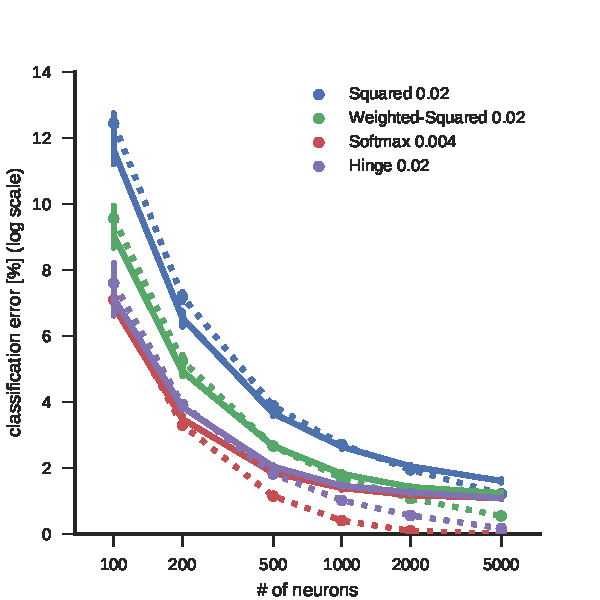
\includegraphics[width=\columnwidth]{mnist_compare_decoders.pdf}
  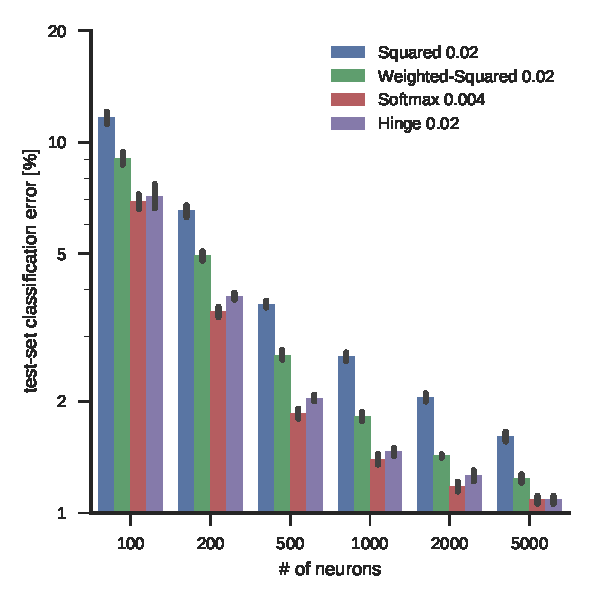
\includegraphics[width=4in]{mnist_compare_decoders_testbar.pdf}
  \captionb{Comparison of loss functions for varying numbers of neurons.}{
    The amount of regularization is chosen optimally for each loss function
    based on \fig{nef-regularization}.
    For all numbers of neurons, softmax loss and hinge loss perform the best.
    They perform equally well for large numbers of neurons,
    but softmax loss performs better for small numbers.
    This may be because the hinge loss regularization was chosen based
    on 5000 neurons, and may not be optimal for fewer neurons.
    Weighted squared loss performs significantly better than
    unweighted squared loss for all numbers of neurons,
    though never as well as softmax or hinge loss.
    Error bars show 95\% confidence intervals of the
    mean classification error across 10 trials.
  }
  \figlabel{nef-decoders}
\end{figure}

\fig{nef-decoders} compares the loss functions with optimal regularization,
across different numbers of hidden neurons.
For large numbers of neurons,
hinge loss and softmax loss perform equally well.
For fewer neurons, softmax tends to perform better,
though this result may not always be statistically significant
(see 95\% confidence interval bars).
This difference between hinge loss and softmax loss could be because
the regularization for hinge loss is chosen based on 5000 hidden neurons,
and that amount of regularization is no longer optimal for fewer neurons.
Since hinge loss is generally more affected by regularization than softmax loss
(see \fig{nef-regularization}), this would put softmax loss ahead for fewer neurons.
This could suggest that softmax loss is more robust
across varying numbers of neurons.

The other key result from this figure is that weighted squared loss
performs significantly better than its unweighted counterpart
across all numbers of neurons,
but not as well as softmax loss or hinge loss.
This can be explained by how well each loss function is able to
fit the training data (see \fig{nef-regularization}).
For lower amounts of regularization,
softmax loss and hinge loss are able to achieve almost zero classification error,
that is they are able to fully fit the training data.
The squared loss methods, on the other hand,
still misclassify many training examples,
likely due to the drawbacks of squared loss as described in \scn{squaredloss}.
However, weighted squared loss performs much better on the training data
than unweighted squared loss,
allowing it to perform better on the test data as well.


%% %% With the optimal amount of regularization,
%% hinge loss performs the best,
%% followed by softmax loss,
%% then both variants of the weighted least squares loss.
%% The plain least squares loss performs the worst,
%% considerably worse than the others.
%% Since plain least squares loss is still the norm
%% for many recent fixed-encoder networks \parencite[\eg/][]{McDonnell2015},
%% this suggests that better loss functions could considerably improve
%% current state-of-the-art results.


\subsection{Spiking}

\begin{figure}
  \centering
  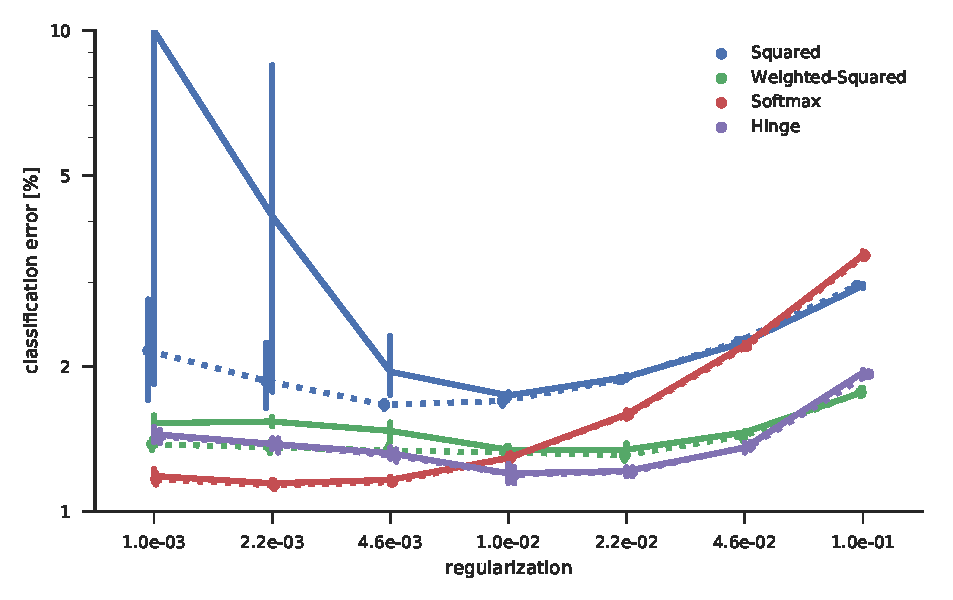
\includegraphics[width=6.35in]{mnist_compare_decoder_spiking_regularization.pdf}
  \captionb{Effects of regularization on spiking networks with 5000 hidden units.}{
    Solid lines show spiking network test-set error,
    dotted lines show rate network test-set error.
  }
  \figlabel{nef-spikingregularization}
\end{figure}

By substituting spiking LIF neurons for the rate LIF neurons used for training,
we can create networks of spiking neurons for classification.
Regularization has an even greater benefit on spiking networks,
as shown in \fig{nef-spikingregularization}.
This is because not only does regularization help with generalization
from the testing set to the training set,
it also helps reduce the variance caused by spikes
by penalizing large decoding weight magnitudes.
Large decoding weights amplify the variance caused by spiking neurons
by making the output much more dependent on some neurons over others.
When decoding weight magnitudes are more uniform---%
as encouraged by $L_2$-regularization---%
the spiking variance from different neurons tends to cancel out,
leading to less variance in the output.

Regularization is most important for the unweighted squared loss classifier
(\fig{nef-spikingregularization}, blue line).
When this loss function is not regularized,
it sometimes puts large weights on some neurons over others.
By doing so, it can better exploit some patterns it finds in the training data;
for example, one neuron having a slightly higher activation than another neuron
might indicate a particular class,
such that the amplified difference between these two neurons
can be used in the classifier.
However, pitting one neuron against another like this
is often not robust when we move to spiking neurons,
since spikes are variable and dynamic, where rates are not.
Thus, the unregularized squared loss classifier sometimes fails catastrophically,
getting $> 20\%$ error in spiking neurons
despite achieving $\sim 2\%$ error in rate neurons.
This only seems to happen one or two times in ten;
the rest of the time, the spiking error is reasonably close (within 1\%)
to the rate-neuron error.
This occasional catastrophic failure is why the unregularized squared loss
has such high mean errors in \fig{nef-spikingregularization},
and why the error bars are so large.

% softmax and hinge loss margins make regularization less necessary
Softmax loss and hinge loss, by contrast,
hardly benefit at all from regularization
when moving from rate neurons to spiking neurons;
in \fig{nef-spikingregularization},
the rate-neuron and spiking-neuron curves are almost identical.
This is probably because both softmax loss and hinge loss
increase the margin between the correct class and the other classes,
which means that variance in the spiking output
will have less of an effect on the classification.
Even though hinge loss does benefit significantly from regularization,
since it decreases the magnitude of the weights
and thereby increases the effective margin enforced by the loss function,
this benefit appears to apply equally to the rate-neuron case
as the spiking neuron case,
as evidenced by both curves being so close in \fig{nef-spikingregularization}.
Thus, for hinge loss, the optimal amount of regularization
for rate neurons is also the optimal amount of regularization for spiking neurons.

\begin{figure}
  \centering
  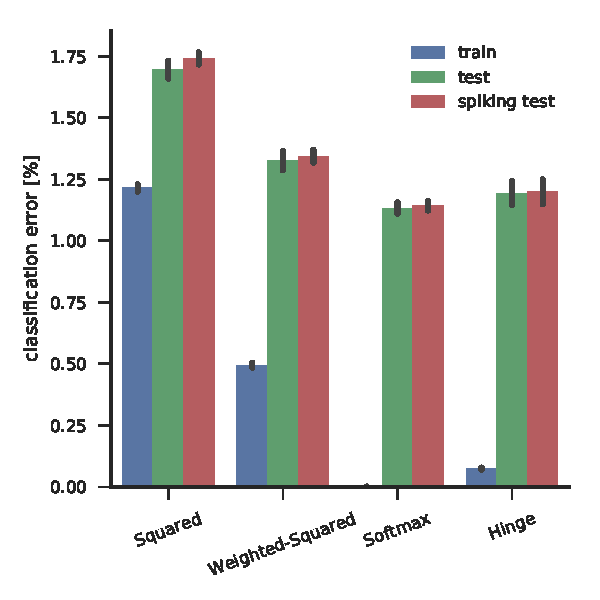
\includegraphics[width=4in]{mnist_compare_decoder_spiking.pdf}
  \captionb{Comparison of loss functions for spiking networks.}{
    The train, test, and spiking classification errors for each loss function
    using 5000 Gabor-encoder neurons on the MNIST task.
    Error bars show 95\% confidence intervals of the mean over 10 trials.
    On average, softmax loss performs the best,
    though it is not statistically much different than hinge loss.
  }
  \figlabel{nef-spikingdecoders}
\end{figure}

\fig{nef-spikingdecoders} shows the best results (optimal $\rho$)
for each loss function.
Softmax loss performs the best, both on the training and test sets,
and in spiking neurons, with hinge loss a close second.
Furthermore, the implicit and explicit margins enforced by
softmax and hinge loss, respectively,
help them both to generalize to spiking neurons very well.
By contrast, unweighted squared loss makes a number more errors
when using spiking neurons,
even with the optimal amount of regularization as shown in the figure.

I chose the spike rates of the network to be low enough
that they are both on the same order of magnitude as cortical spike rates,
and to allow them to be implemented on neuromorphic hardware.
Furthermore, low spike rates also help demonstrate that the network
is truly robust to the variability caused by spikes;
neurons with high spike rates, when filtered by a synapse,
end up having very low variability in their output,
and act essentially as rate neurons.
The neurons in the spiking networks presented here all had
average neuron firing rates between 17 and 19 Hz.
The firing was somewhat sparse, with an average of 30-32\% of neurons
responding to any particular input.
Thus, the average firing rate of neurons when they are responding is higher,
in the 58-60 Hz range.


\subsection{Computation time}

\begin{figure}
  \centering
  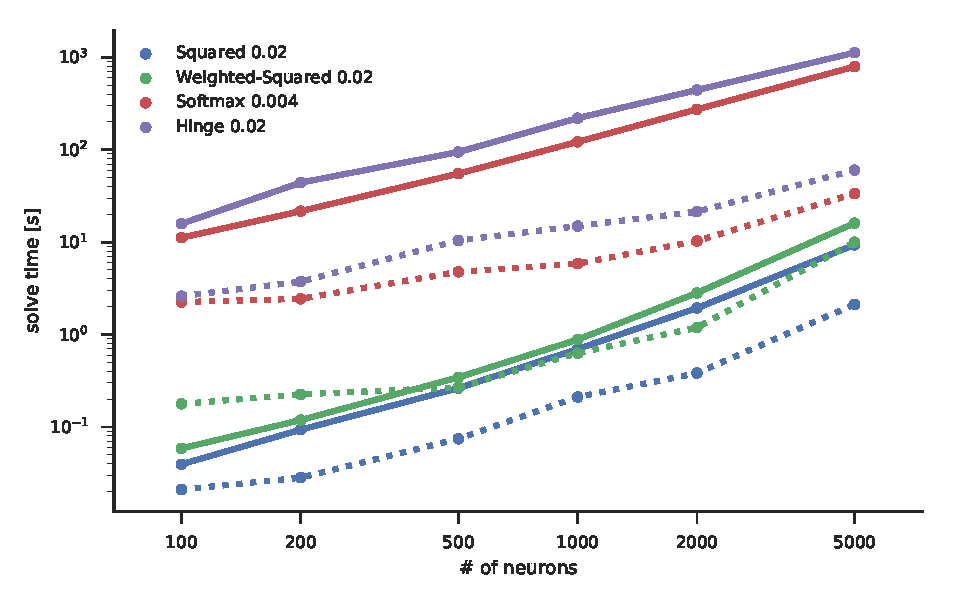
\includegraphics[width=6.35in]{mnist_compare_solve_time.pdf}
  \captionb{Training time for the various loss functions.}{
    Solid lines show CPU times, dotted lines show GPU times.
    CPU: OpenBLAS on Intel Xeon E5-1650 @ 3.5GHz (6 cores),
    GPU: clBLAS on NVIDIA GTX 980 @ 1126 MHz (2048 cores)
    %% GPU: clBLAS on NVIDIA GTX 980 @ 4.6 TFLOPs
  }
  \figlabel{nef-solvetime}
\end{figure}

\fig{nef-solvetime} shows the time required for training
for various loss functions on both CPU (solid line) and GPU (dotted line).
Both axes are logarithmic,
so the slope of the line indicates how the computation speed scales
with the number of neurons,
with a slope of unity corresponding to linear scaling.

The solvers can be grouped into two categories:
the squared loss solvers, which both use direct solution methods;
and the softmax and hinge loss solvers, which use iterative solution methods.
Given the number of training examples $M$ (60000 for the MNIST dataset used here),
the number of neurons $N$,
and the number of categories $C$ (10 for MNIST),
we can compute order of magnitude
of the theoretical computational complexity for each method.
The direct methods both involve computing a correlation matrix
between all the neurons over all the examples,
which is $O(MN^2)$.
The $N$-dimensional linear system corresponding to this matrix
then has to be solved; this is $O(N^3)$.
These are the two main steps in both the squared loss algorithms.
All the other steps in these algorithms are of lower orders (\eg/ $O(N^2)$).
The order of the squared loss algorithm is thus $O(MN^2 + N^3)$.
Since the weighted squared loss requires solving
a separate system for each output category,
its order is $O(CMN^2 + CN^3)$.
Using the method described in \app{wlls},
this can be reduced to $O(2MN^2 + CN^3)$.
Since it is often the case that $M \gg N$,
these methods are often dominated by the $O(MN^2)$ term;
that is, the matrix-matrix multiply is the most costly operation.
This means that as we vary $N$, we expect the solvers to vary as $N^2$.

In \fig{nef-solvetime},
we see that the squared solvers actually vary as somewhere
between $N$ and $N^2$ on the CPU (solid blue and green lines).
This is likely because as the size of the computation grows,
overhead costs become less significant,
and computations can be performed at closer to optimal speed.
A detailed examination of the plot shows that as $N \to 5000$,
the slope of both lines approaches $N^2$.
The weighted squared solver is consistently slightly slower
than the squared solver,
as one would expect from the analysis above.
This effect becomes slightly more pronounced as $N$ increases,
because as $N \to 5000$, $CN \to M$,
which means that the $O(CN^3)$ term begins to compete with the $O(2MN^2)$ term.
I expect this speed difference to become more pronounced as $N$ continues to increase.

A theoretical analysis for the softmax and hinge loss algorithms
is more difficult to perform,
because these algorithms have one important unknown:
the number of iterations required for convergence.
The main factor that affects the number of iterations
is the conditioning of the problem,
where better-conditioned problems will converge more quickly.
Thus, the amount of regularization can have a significant effect
on the convergence;
here, I used the optimal regularization as determined previously,
since this seemed like the most pertinent choice.
What we can do is compute the computational complexity
of the cost and gradient computations that happen each iteration.
For both algorithms,
the computational complexity of a cost-gradient computation
is dominated by two matrix-matrix products,
one between the neuron activities and the parameters to determine the outputs,
and the second between the neuron activities and the output derivatives
to determine the parameter gradients.
Both of these operations are $O(MNC)$,
making the cost of one step $O(2MNC)$.
Thus, assuming the number of required iterations
is independent of the number of neurons,
both these algorithms should scale linearly with the number of neurons $N$.

Looking at the time taken on the CPU by softmax (red solid line)
and hinge loss (purple solid line) in \fig{nef-solvetime},
these two functions do appear to scale almost linearly
with the number of neurons
(a careful examination reveals that they are slightly supralinear).
Hinge loss consistently takes more time than softmax loss;
this appears to be because hinge loss often runs for more iterations
than softmax loss.

All of these solution methods are at least partially parallelizable.
All the matrix-matrix products can be parallelized,
reducing some of the most costly operations for all algorithms.
The only costly operation that I have not parallelized here
is the solution of the linear system(s) in the direct methods.\footnote{
  Parallel algorithms do exist for Cholesky factorization,
  and have been implemented in OpenCL
  (see \url{http://icl.cs.utk.edu/magma/software/view.html?id=190}).
  However, this code has not been ported to work with PyOpenCL,
  as far as I am aware.
  Doing so would not be difficult,
  but since solving the linear systems is typically the less costly part
  of the algorithms explored here,
  I did not take the time to do so myself.}
As \fig{nef-solvetime} shows,
running these algorithms on the GPU is almost always faster than on the CPU,
with the exception being the weighted squared loss for smaller number of neurons.
Overall, weighted squared loss receives the least benefit from the GPU,
since it relies most heavily on solving linear systems,
which I am not running on the GPU.
A close examination shows that for larger number of neurons,
the scaling with $N$ is the same on the GPU as on the CPU.
This is as expected, since larger $N$ are able to utilize all GPU cores,
thus increasing $N$ past that threshold will scale the computation time
as per the theoretical analysis.

\begin{table}
  \centering
  \begin{tabular}{lrrr}
    Core method           & Single $\rho$ & Many (30) $\rho$ & LOO method \\\hline
    Squared loss          & 16.07 s       & 482.10 s         & 81.97 s \\
    Weighted squared loss & 25.63 s       & 768.90 s         & 1054.06 s \\
  \end{tabular}
  \captionb{Computation time of the LOO cross-validation method.}{
    As compared with brute-force validation on a separate validation set.
    The first column shows the cost of running either method for a single
    value of the regularization parameter $\rho$, for 5000 neurons.
    The second column shows the cost of running the single method 30 times,
    which would be the approximate cost of doing cross validation
    on a separate validation set by grid search.
    The third column shows the cost of the LOO method.
    For unweighted squared loss, the LOO method offers potential savings,
    but it performs worse on the weighted squared loss.
    }
  \tablabel{rifkin}
\end{table}

\tab{rifkin} shows the results of testing the computation time
of the \textcite{Rifkin2007} method
for finding the optimal regularization parameter using the LOO error.
When using squared loss, the cost of the LOO method is roughly five times
that of the basic method.
This additional cost is mainly due to computing $\mat P = \mat A \mat Q$,
which is an $O(MN^2)$ operation like $\mat A \mat A^T$,
but unlike the computation of $\mat A \mat A^T$,
the result is not symmetric, so it requires twice the computation time.
The remaining computational costs are due largely to the matrix-vector
products required for testing each different value of $\rho$.
Despite this large increase in computation time,
the LOO method is still more computationally efficient than
running the basic method 30 times to test sufficient values of $\rho$
to get a decent estimate using a separate validation set.
If instead of using grid search to perform the cross-validation
on a separate validation set,
we used an optimization method such as golden-section search,
roughly 15 test values of $\rho$ would be required instead of 30
(based on observations from testing the LOO cross-validation).
This would cut the times of the middle column in half,
though for unweighted squared error, the LOO method would still perform better.

For weighted squared error, the LOO method is much more costly.
This is because we now require $C$ additional matrix-matrix products of $O(MN^2)$,
in addition to the other computations required for computing the LOO error.
This results in the LOO method being sub-optimal for weighted squared error,
taking more time than a brute-force grid-search cross-validation
on a separate validation set.


\section{Discussion}

Of the encoder generation methods examined in \scn{enc-results},
Gabor filters perform best (\fig{nef-encoder-summary}).
This is in spite of the fact that they are tuned for general image statistics,
whereas the encoders yielded by the CIW and CD methods
are tuned for the specific dataset (MNIST, in this case).
This suggests that tuning encoders to each specific dataset is not necessary,
at least for the first layer of hidden neurons.
While using Gabor filters for encoding is not a new idea,
the fact that they perform better than the newer CIW and CD methods
suggests that the utility of these new methods is limited
in terms of generating first-layer encoders.

\fig{nef-decoders} shows that unweighted squared loss performs worst
of all the loss functions examined.
Since it is still the norm
for many recent fixed-encoder networks \parencite[\eg/][]{McDonnell2015},
these results suggest better loss functions could considerably improve
current state-of-the-art results.
Weighted squared loss is computable for a relatively small cost
over unweighted squared loss (see \app{wlls}),
and even softmax loss or hinge loss minimization can be performed
in a very reasonable amount of time on a GPU (\fig{nef-solvetime}).

Softmax loss appears to be the overall best loss function
for fixed-encoding SLFNs for MNIST.
Not only does it yield the best results
(though hinge loss is not significantly worse, see \fig{nef-spikingdecoders}),
it is also the least sensitive to the amount of regularization
(Figures \figref{nef-regularization} and \figref{nef-spikingregularization}).
The main downside to softmax loss is that
it requires more computation time than squared loss methods
(\fig{nef-solvetime}),
since a closed-form solution is not possible.

All of the loss functions presented in this chapter
can theoretically be used with the Prescribed Error Sensitivity (PES)
learning rule \parencite{MacNeil2011,Bekolay2013},
a derivative-free variant of the delta rule adapted for NEF networks.
This would allow decoders to be learned online in a biologically-plausible manner.
Some loss functions might be more amenable to this than others.
For example, the squared loss has a linear derivative,
and is the standard for both online and offline learning in NEF networks.
The weighted squared loss also has a linear derivative,
but the weighting terms will require scaling the learning on different decoders
depending on the target class of the digit.
The softmax and hinge loss both have nonlinear derivatives.
The softmax loss requires computing a softmax function,
which requires normalization and may not be straightforward in spiking neurons.
Hinge loss requires computing an argmax function,
which again is not straightforward,
though there is evidence for such functions being computed
in specialized regions such as the basal ganglia \parencite{Redgrave1999}.

There is a significant drawback to the methods examined in this chapter:
they may not be able to generalize to more difficult datasets,
and even if they can, they may require so many hidden neurons to perform well
that training them becomes infeasible.
So far, fixed-encoding networks have predominantly been tested
on the MNIST dataset.
This dataset does not have the complexity of other,
more realistic datasets like CIFAR-10.
The visual appearance of MNIST digits is very simple,
with trivially distinguishable foreground and background.
The categories are also very distinguishable,
depending on only a few simple visual features.

For more complex datasets,
it is unlikely that SLFNs will be able to perform well.
I tried the networks described in this chapter on the CIFAR-10 dataset,
using 15000 hidden units as well as data augmentation,
and achieved 36\% test error (27\% train error),
which is nowhere near the state-of-the-art.
The best performance for fixed-encoding networks on the CIFAR-10 dataset
is by \textcite{McDonnell2015a},
who use a two-layer fixed-encoding network
with a 96-filter convolution and pooling layer
followed by a 40000 hidden unit fully-connected layer,
to achieve 24.14\% test error.
An identical network achieves 3.96\% test error on the SVHN dataset.
Multilayer networks, particularly those with convolution and pooling,
make solving problems like translation invariance
much more straightforward than with a single-layer network.
The convolutional filters in this network are taken from the Overfeat
network trained on ImageNet,
thus incorporating significant prior knowledge about what constitutes good
low level features.
Yet even this large fixed-encoding network
using good convolutional features and pooling
is still a ways from the state-of-the-art,
having about twice the level of error on SVHN (3.96\% vs 1.92\%)
and 2.5 times the level of error on CIFAR-10 (24.14\% vs 9.78\%)
as compared with the best networks trained on these datasets
(without data augmentation).
These are significant gaps,
and it is unclear whether fixed-encoding networks
will be able to overcome them.\footnote{
  The only way that I currently think that fixed-encoding networks
  might do well on these more challenging problems
  is by training a deep network on an even more difficult problem (\eg/ ImageNet),
  and then replacing the final (classifier) layer on the deep network
  with a classifier trained using one of the methods discussed in this chapter.
  In other words, using the whole deep network as the fixed encoder.
  In my opinion, this would not demonstrate
  the power of fixed-encoding networks
  (since one has to train a deep network on a much harder dataset first),
  but would rather demonstrate that transfer learning is viable.}


% NEF method cannot work well for some architectures. For example, a
% 30-20-10 network trying to learn a linear transform. Even if the encoders
% map the input data distribution, the optimal encoders also depend on the
% output function distribution, \ie/ there are degrees of freedom in the input
% that do not affect the output.

On a deeper level,
there are limitations to what types of processing a fixed-encoding network
can hope to perform,
even with a data-driven encoding.
For example, take the problem of learning a linear transform $\mat B$
from $m$ dimensions to $n$ dimensions, where $m \gg n$.
Because the input space is so much larger than the output space,
there will be dimensions of the input space that do not affect the output;
we call these invariances,
and mathematically they correspond to the nullspace of $\mat B$.
If we create a network that uses some sort of random encoding of the input space,
or even learns some encoding using unsupervised learning,
the best we can hope to do is to perfectly represent the input space,
ideally in some way that is sparser or otherwise easier to work with
than the inputs themselves.
We can never hope, though,
that this encoding will pick up on any of the invariances in the dataset.
That is because these invariances depend on the transformation $\mat B$,
and without some explicit or implicit knowledge about this transformation,
we cannot hope to learn them.
It may be possible to take advantage of prior or expert knowledge
about the domain to engineer better features;
this would be using explicit knowledge of $\mat B$.
Or we may have access to some of the mappings
from the input space to the output space,
and can use them in a supervised or semi-supervised learning setting;
this would be using implicit knowledge about $\mat B$.
%% If the encoding is simply concerned with representing the input image

% Lighting invariance
An example of real-world invariance is lighting.
The lighting on a scene can greatly affect the image that falls on one's retina,
but does not affect the identity of the objects in the scene.
For the most part, we are able to operate accurately in scenes lit in many different ways.
Human object recognition must therefore be invariant to many types of lighting variation.
For a computational visual system to be successful,
it must also be able to separate lighting variation from other object characteristics
in such a way that object recognition can be lighting invariant.
Since our fixed-encoding network cannot learn this implicitly
from the training data using supervised learning,
this invariance must be engineered in.
Specifically, we must engineer the system
such that the effects of lighting are factored out,
having some hidden nodes that represent lighting
and some that represent other image features.
Explicitly constructing such a system is no mean feat, however,
and some of the best successes so far have come from using
unsupervised methods to learn this decomposition \parencite{Tang2012}.

For fixed-encoding networks to truly be successful, then,
the designers of such networks will explicitly have to build in invariances
such that the classifier at the end of the network
is able to easily separate the different classes.
The convolutional-pooling fixed-encoding networks of \textcite{McDonnell2015a}
are another example of building in such an invariance,
in that case an invariance to translation.
In this chapter, I used explicit knowledge of the image space---%
namely the fact that natural images are well-modeled by Gabor filters---%
to design a fixed-encoding network.
In its own way, this is building invariance into the network:
invariance to individual pixel fluctuations.
I used the prior knowledge that individual pixel values do not matter by themselves,
but it is rather the edges in an image, or the correlations between many adjacent pixels,
that matter.
However, that invariance will not be enough by itself,
and for that matter, neither will building in only lighting invariances
or only translation invariances.
A good object recognition system will have to account for all these invariances,
and under a fixed-encoding system,
it will be up to the system engineers to enumerate them and build them all in.

These challenges are severe,
and are one of the reasons that the computer vision community
has slowly been moving away from traditional computer vision,
where features are hand-engineered,
and tending towards machine learning approaches,
where the features are discovered using supervised learning approaches.
Such approaches are the focus of the next two chapters of this thesis.

%%  LocalWords:  nef feedforward SLFNs MLP Pao Eliasmith Broomhead ij
%%  LocalWords:  SLFN ik kj ELMs Tapson Zhu Toh lifrate gabor gabors
%%  LocalWords:  RFs CIW ki squaredloss lstsq Rosasco wsquaredloss un
%%  LocalWords:  Fieguth wsquare wlls softmaxloss BFGS Liu Scipy ka
%%  LocalWords:  hingeloss dec Rifkin rifkin eigen jj MNC CMN Spaun
%%  LocalWords:  Cao Diehl Bekolay spikingregularization OpenBLAS GTX
%%  LocalWords:  spikingdecoders Xeon clBLAS solvetime CN lrrr SVHN
%%  LocalWords:  Overfeat RBF Olshausen Krizhevsky PES MacNeil
%%  LocalWords:  argmax
